% !TeX encoding = UTF-8
% !TeX spellcheck = es_ES
% !TeX root = DB-Conectors.tex

\begin{table}[H]
    \centering
    \renewcommand\theadfont{\bfseries}
    \setlength{\tabcolsep}{10pt}
    \renewcommand{\arraystretch}{1.5}

    \begin{tabular}{|c|c|c|c|c|}
        \beginConnectorTable{DC Jack 2mm}
        \multirow{3}{*}{\makecell{Macho \\ Plug}}
    
        \connectordata{
            \begin{scope}
                \clip (-1.3,-0.75) rectangle  +(2.6,1.5);
                \node[inner sep=0pt] at (-1.8,-0.8)
                    {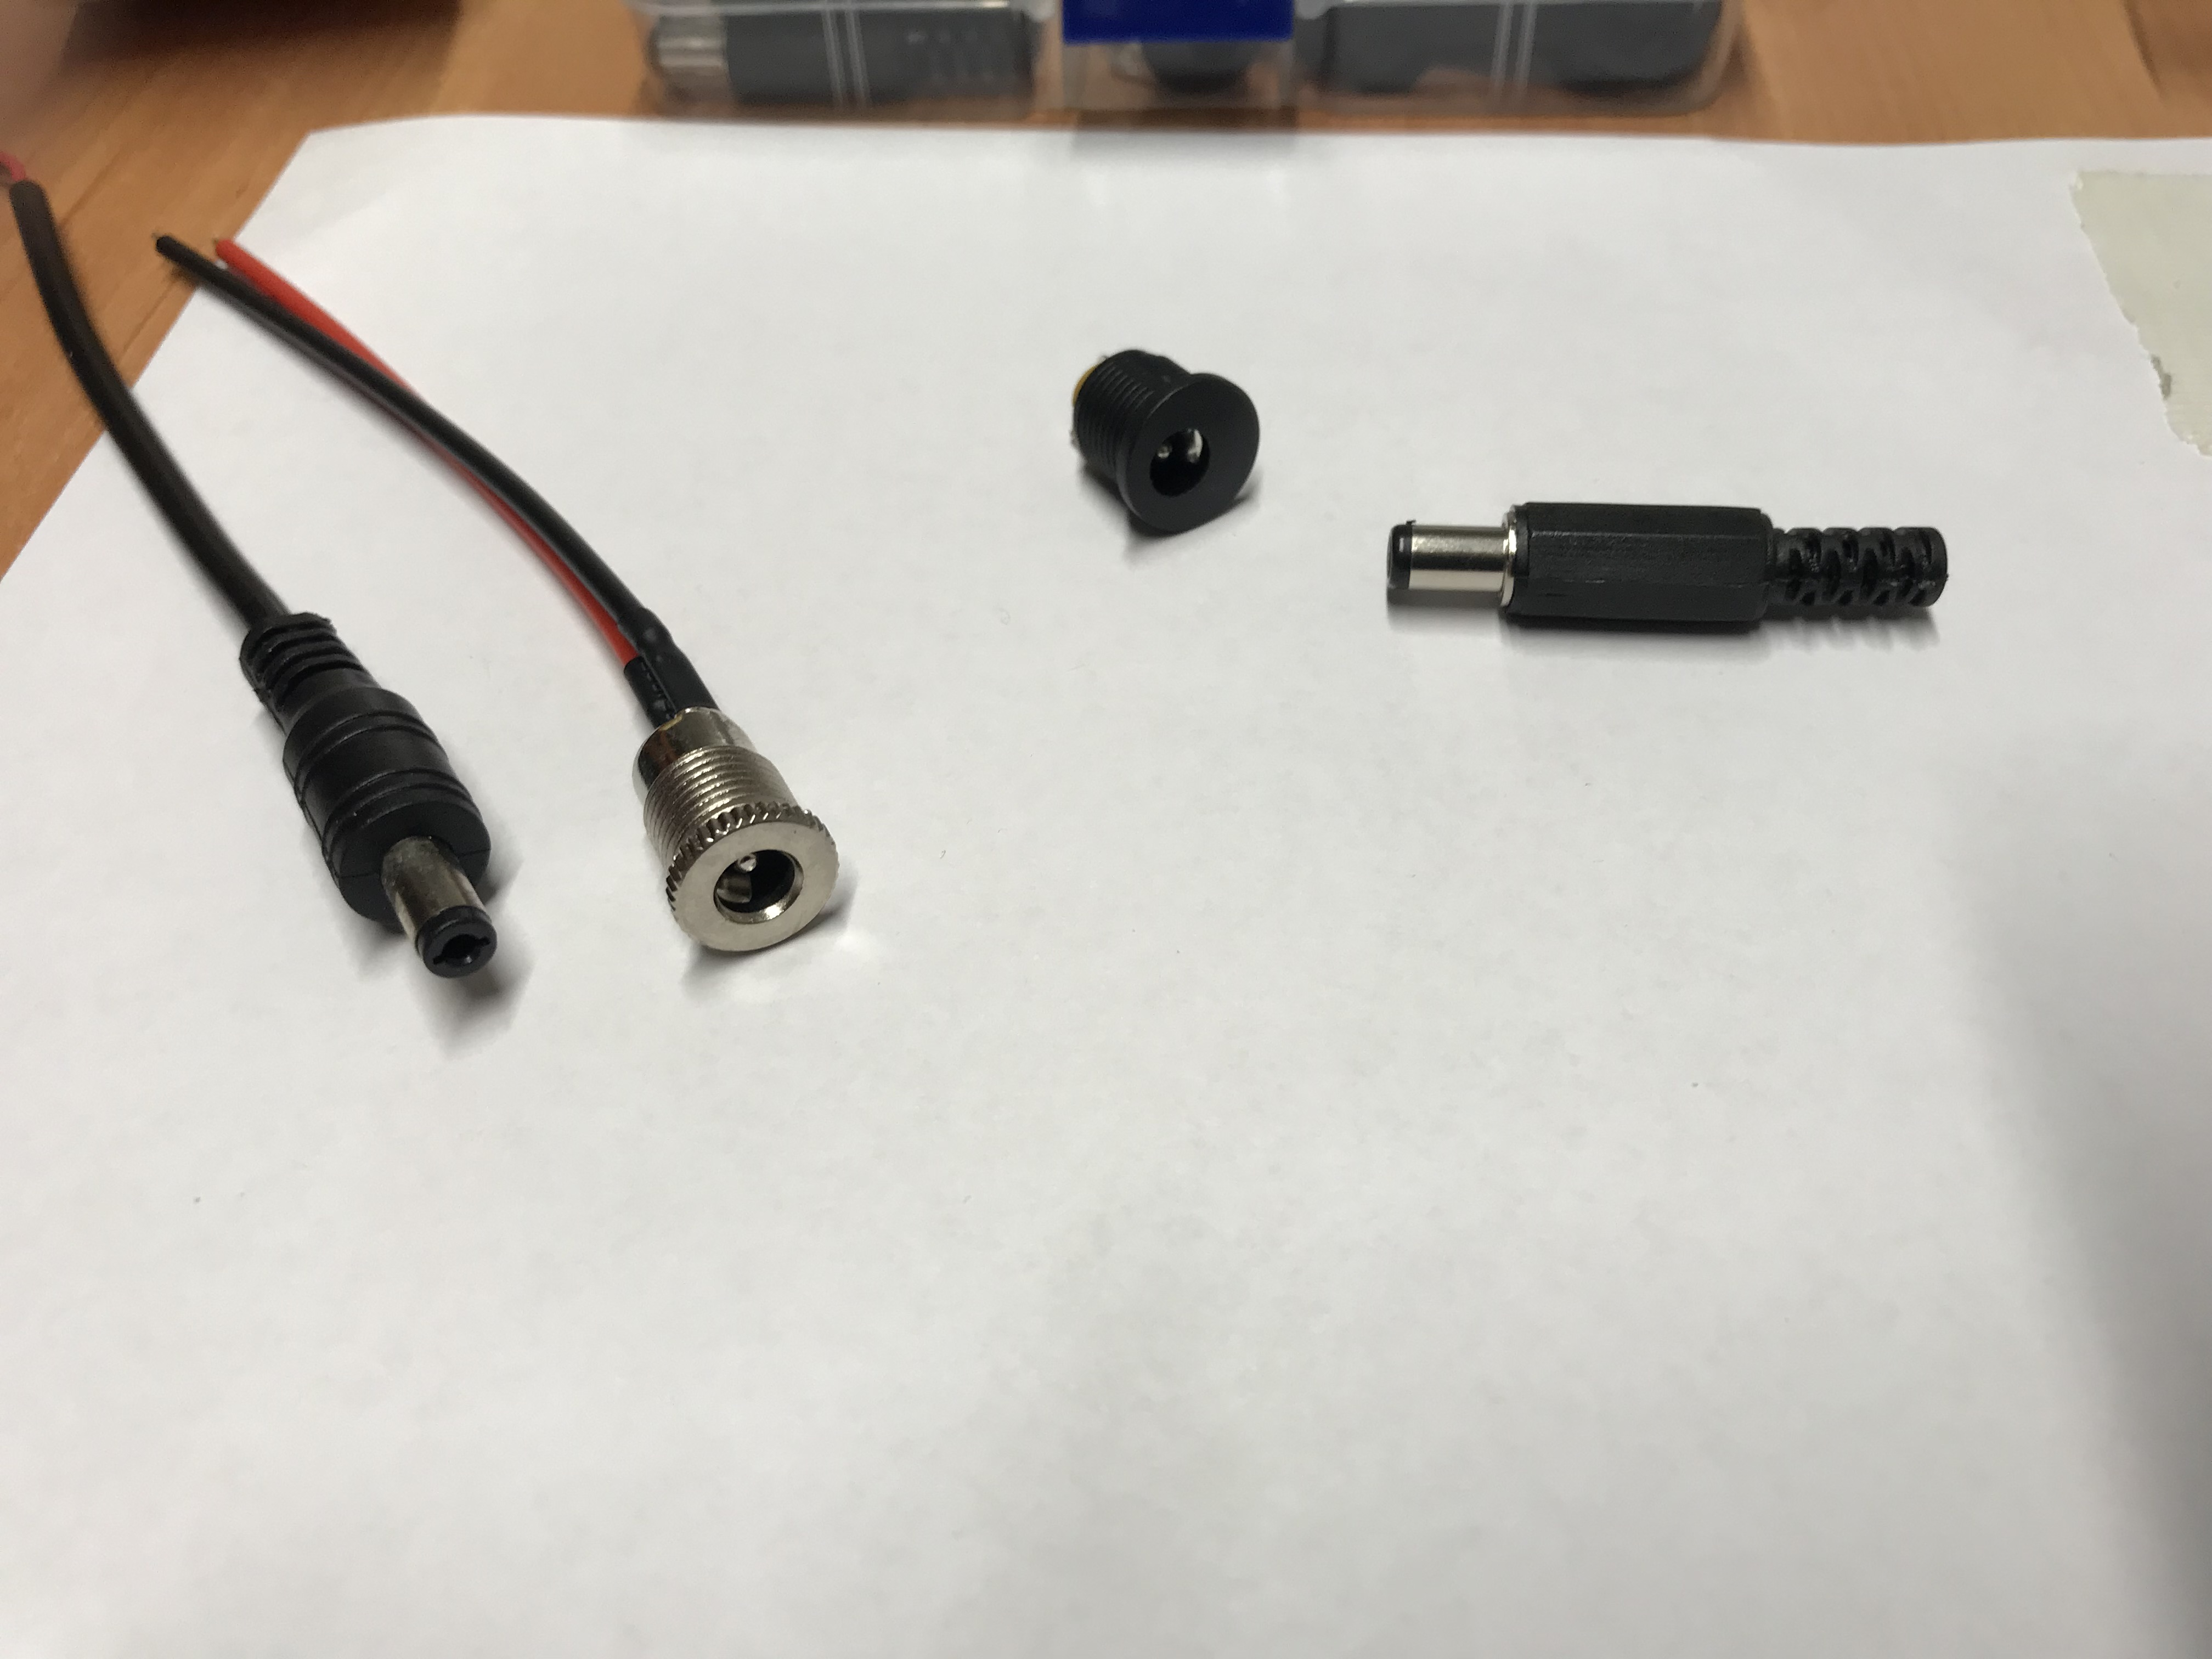
\includegraphics[scale=.05]{pictures/dcJack.jpg}};
            \end{scope}
        }{
            \draw (0,0) rectangle (3,1.5) ;
        }{Amazon}{Sin Id} {24V} {3A}
        \multirow{3}{*}{\makecell{Hembra \\ Socket}}
        \connectordata{
            \begin{scope}
                \clip (-1,-0.75) rectangle  +(2,1.5);
                \node[inner sep=0pt] at (-0.2,-1.7)
                    {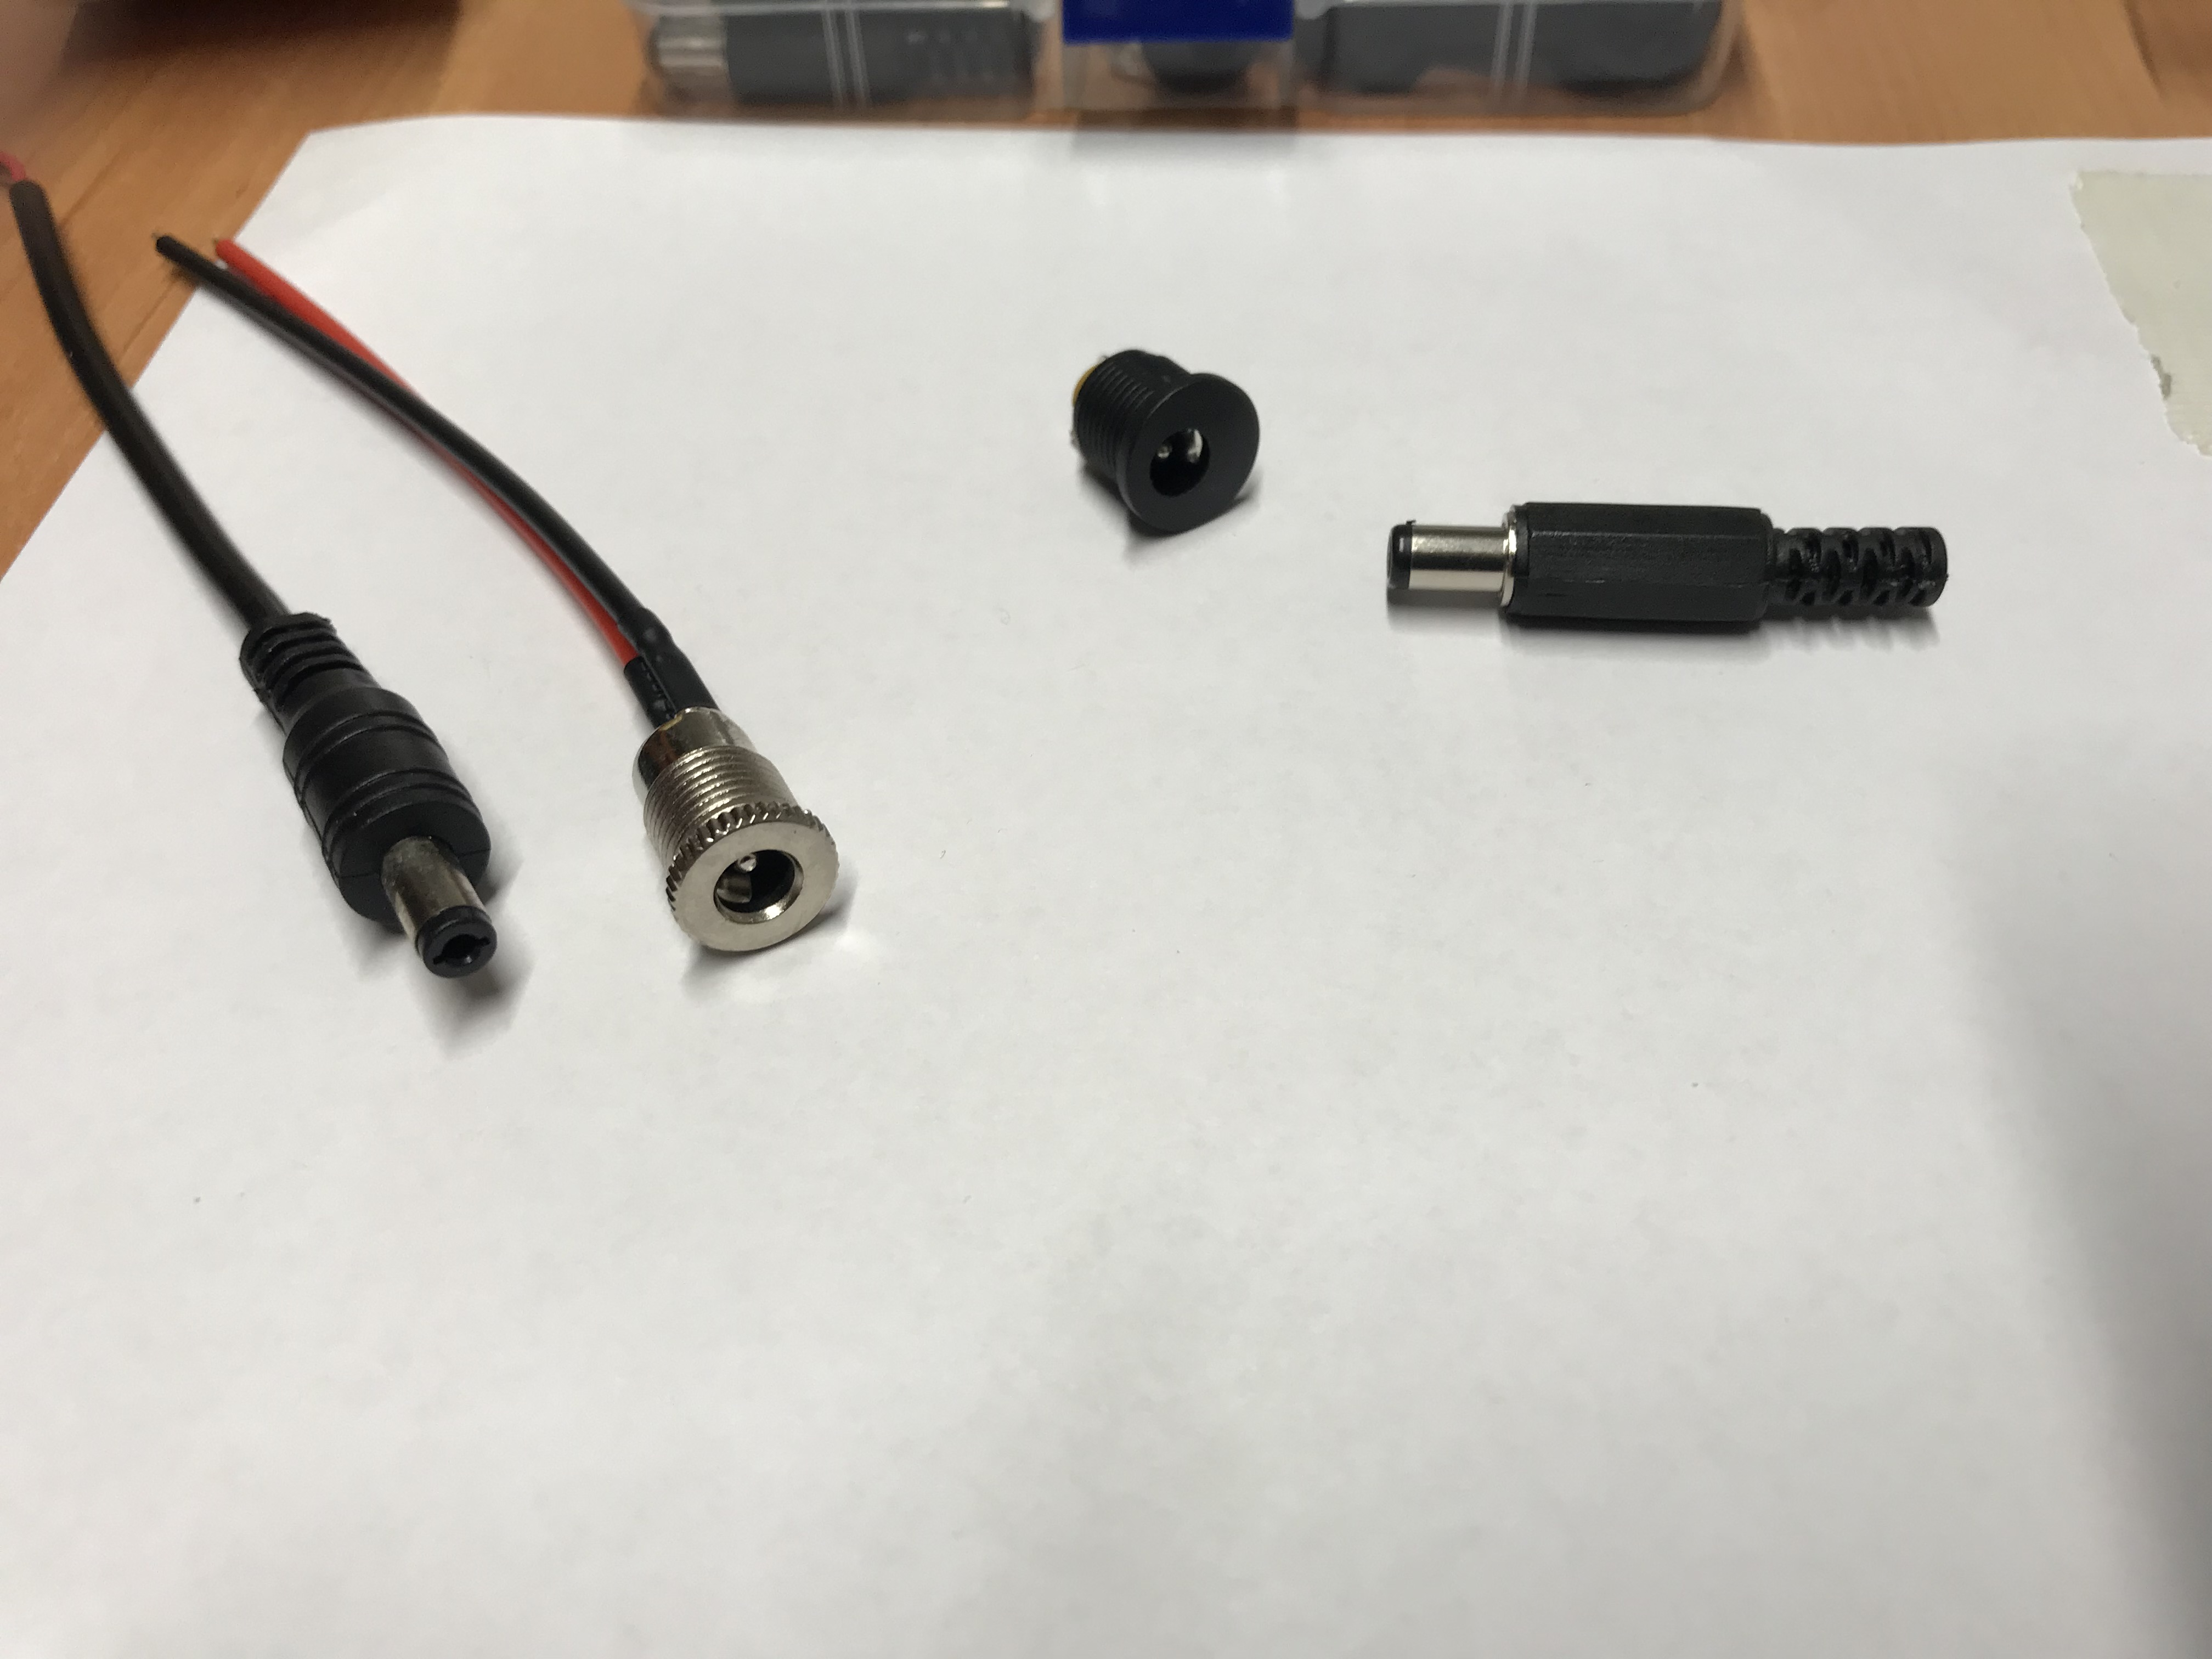
\includegraphics[scale=.07]{pictures/dcJack.jpg}};
            \end{scope}
        }{
            \draw (0,0) rectangle (3,1.5) ;
        }{Amazon}{Sin Id} {24V} {3A}

        \multicolumn{5}{|l|}{\makecell[l]{
            \tabitem Incluye tuerca para sujetar a panel \\
            \tabitem Incluye protector de goma
        }} \\
        \hline
    \end{tabular}
    \caption{Jack 2mm Amazon}
    \label{tab:DcJack1}
\end{table}

\begin{table}[H]
    \centering
    \renewcommand\theadfont{\bfseries}
    \setlength{\tabcolsep}{10pt}
    \renewcommand{\arraystretch}{1.5}

    \begin{tabular}{|c|c|c|c|c|}
        \beginConnectorTable{DC Jack 2mm}
        \multirow{3}{*}{\makecell{Macho \\ Plug}}
    
        \connectordata{
            \begin{scope}
                \clip (-1,-0.65) rectangle  +(2,1.3);
                \node[inner sep=0pt, rotate=60] at (1.3,2)
                    {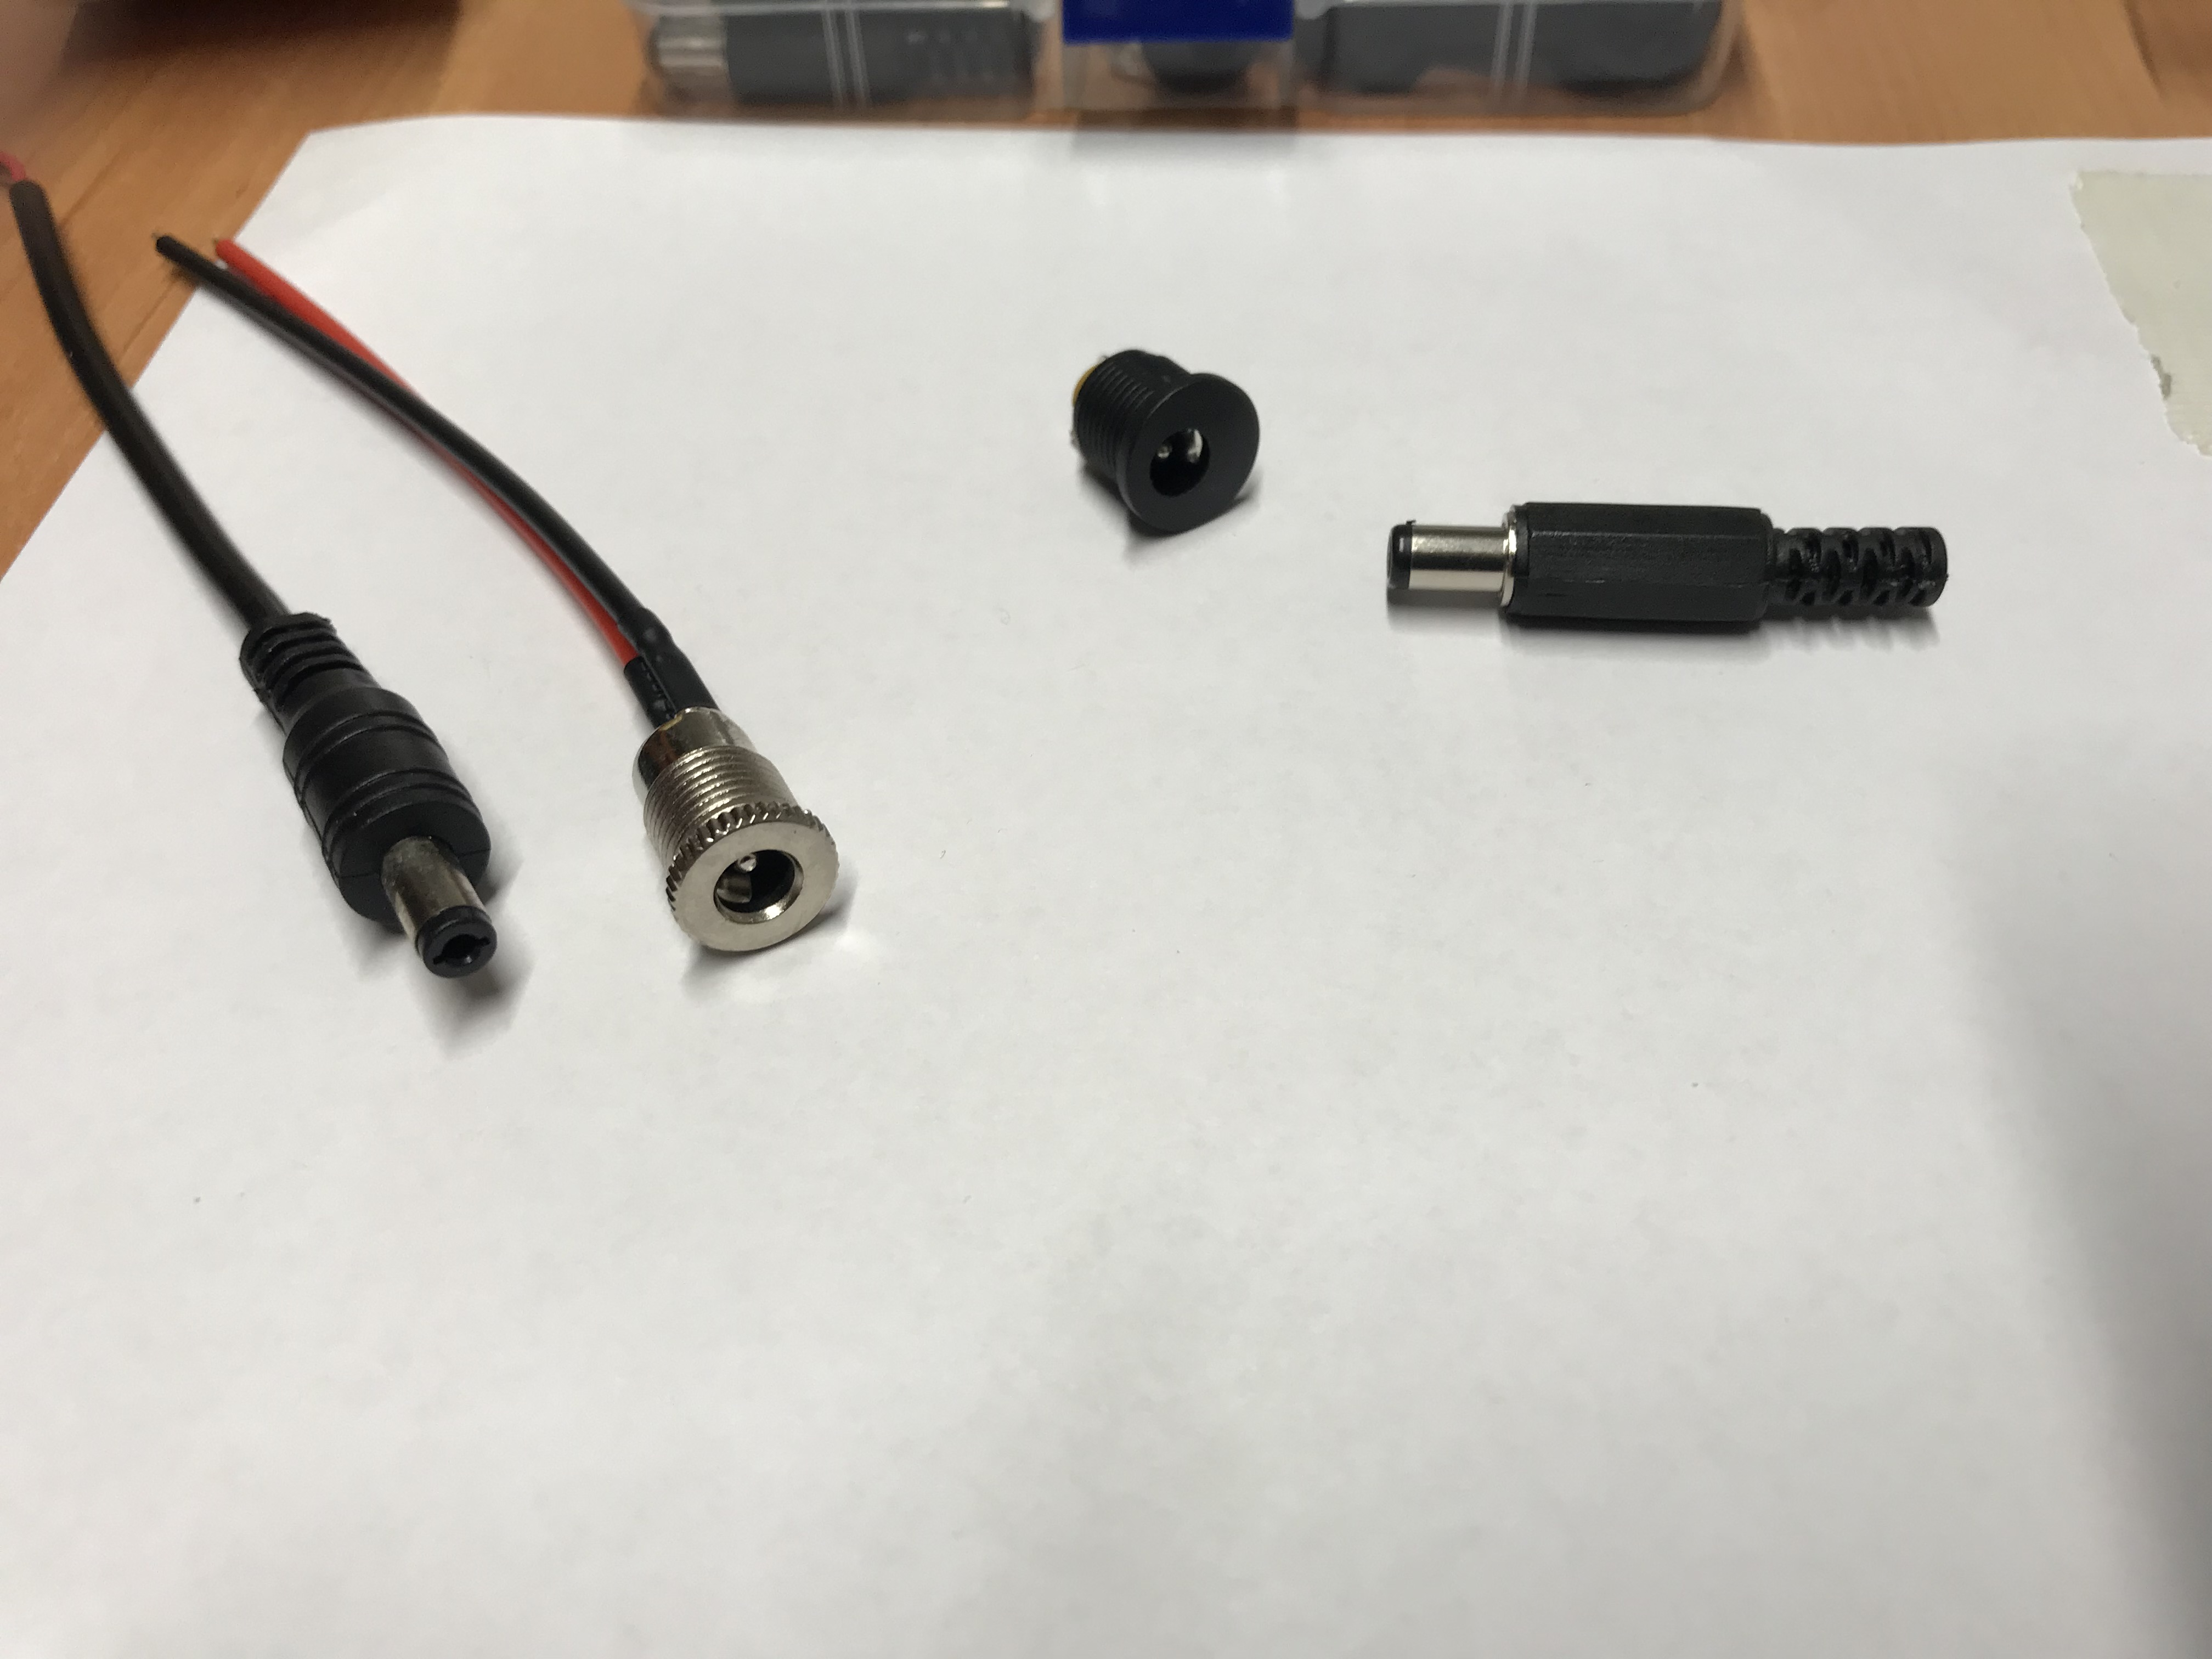
\includegraphics[scale=.05]{pictures/dcJack.jpg}};
            \end{scope}
           
        }{
            \draw (0,0) rectangle (3,1.5) ;
        }{Amazon}{Sin Id} {24V} {3A}
        \multirow{3}{*}{\makecell{Hembra \\ Socket}}
        \connectordata{
            \begin{scope}
                \clip (-1,-0.65) rectangle  +(2,1.3);
                \node[inner sep=0pt, rotate=60] at (0.9,1)
                    {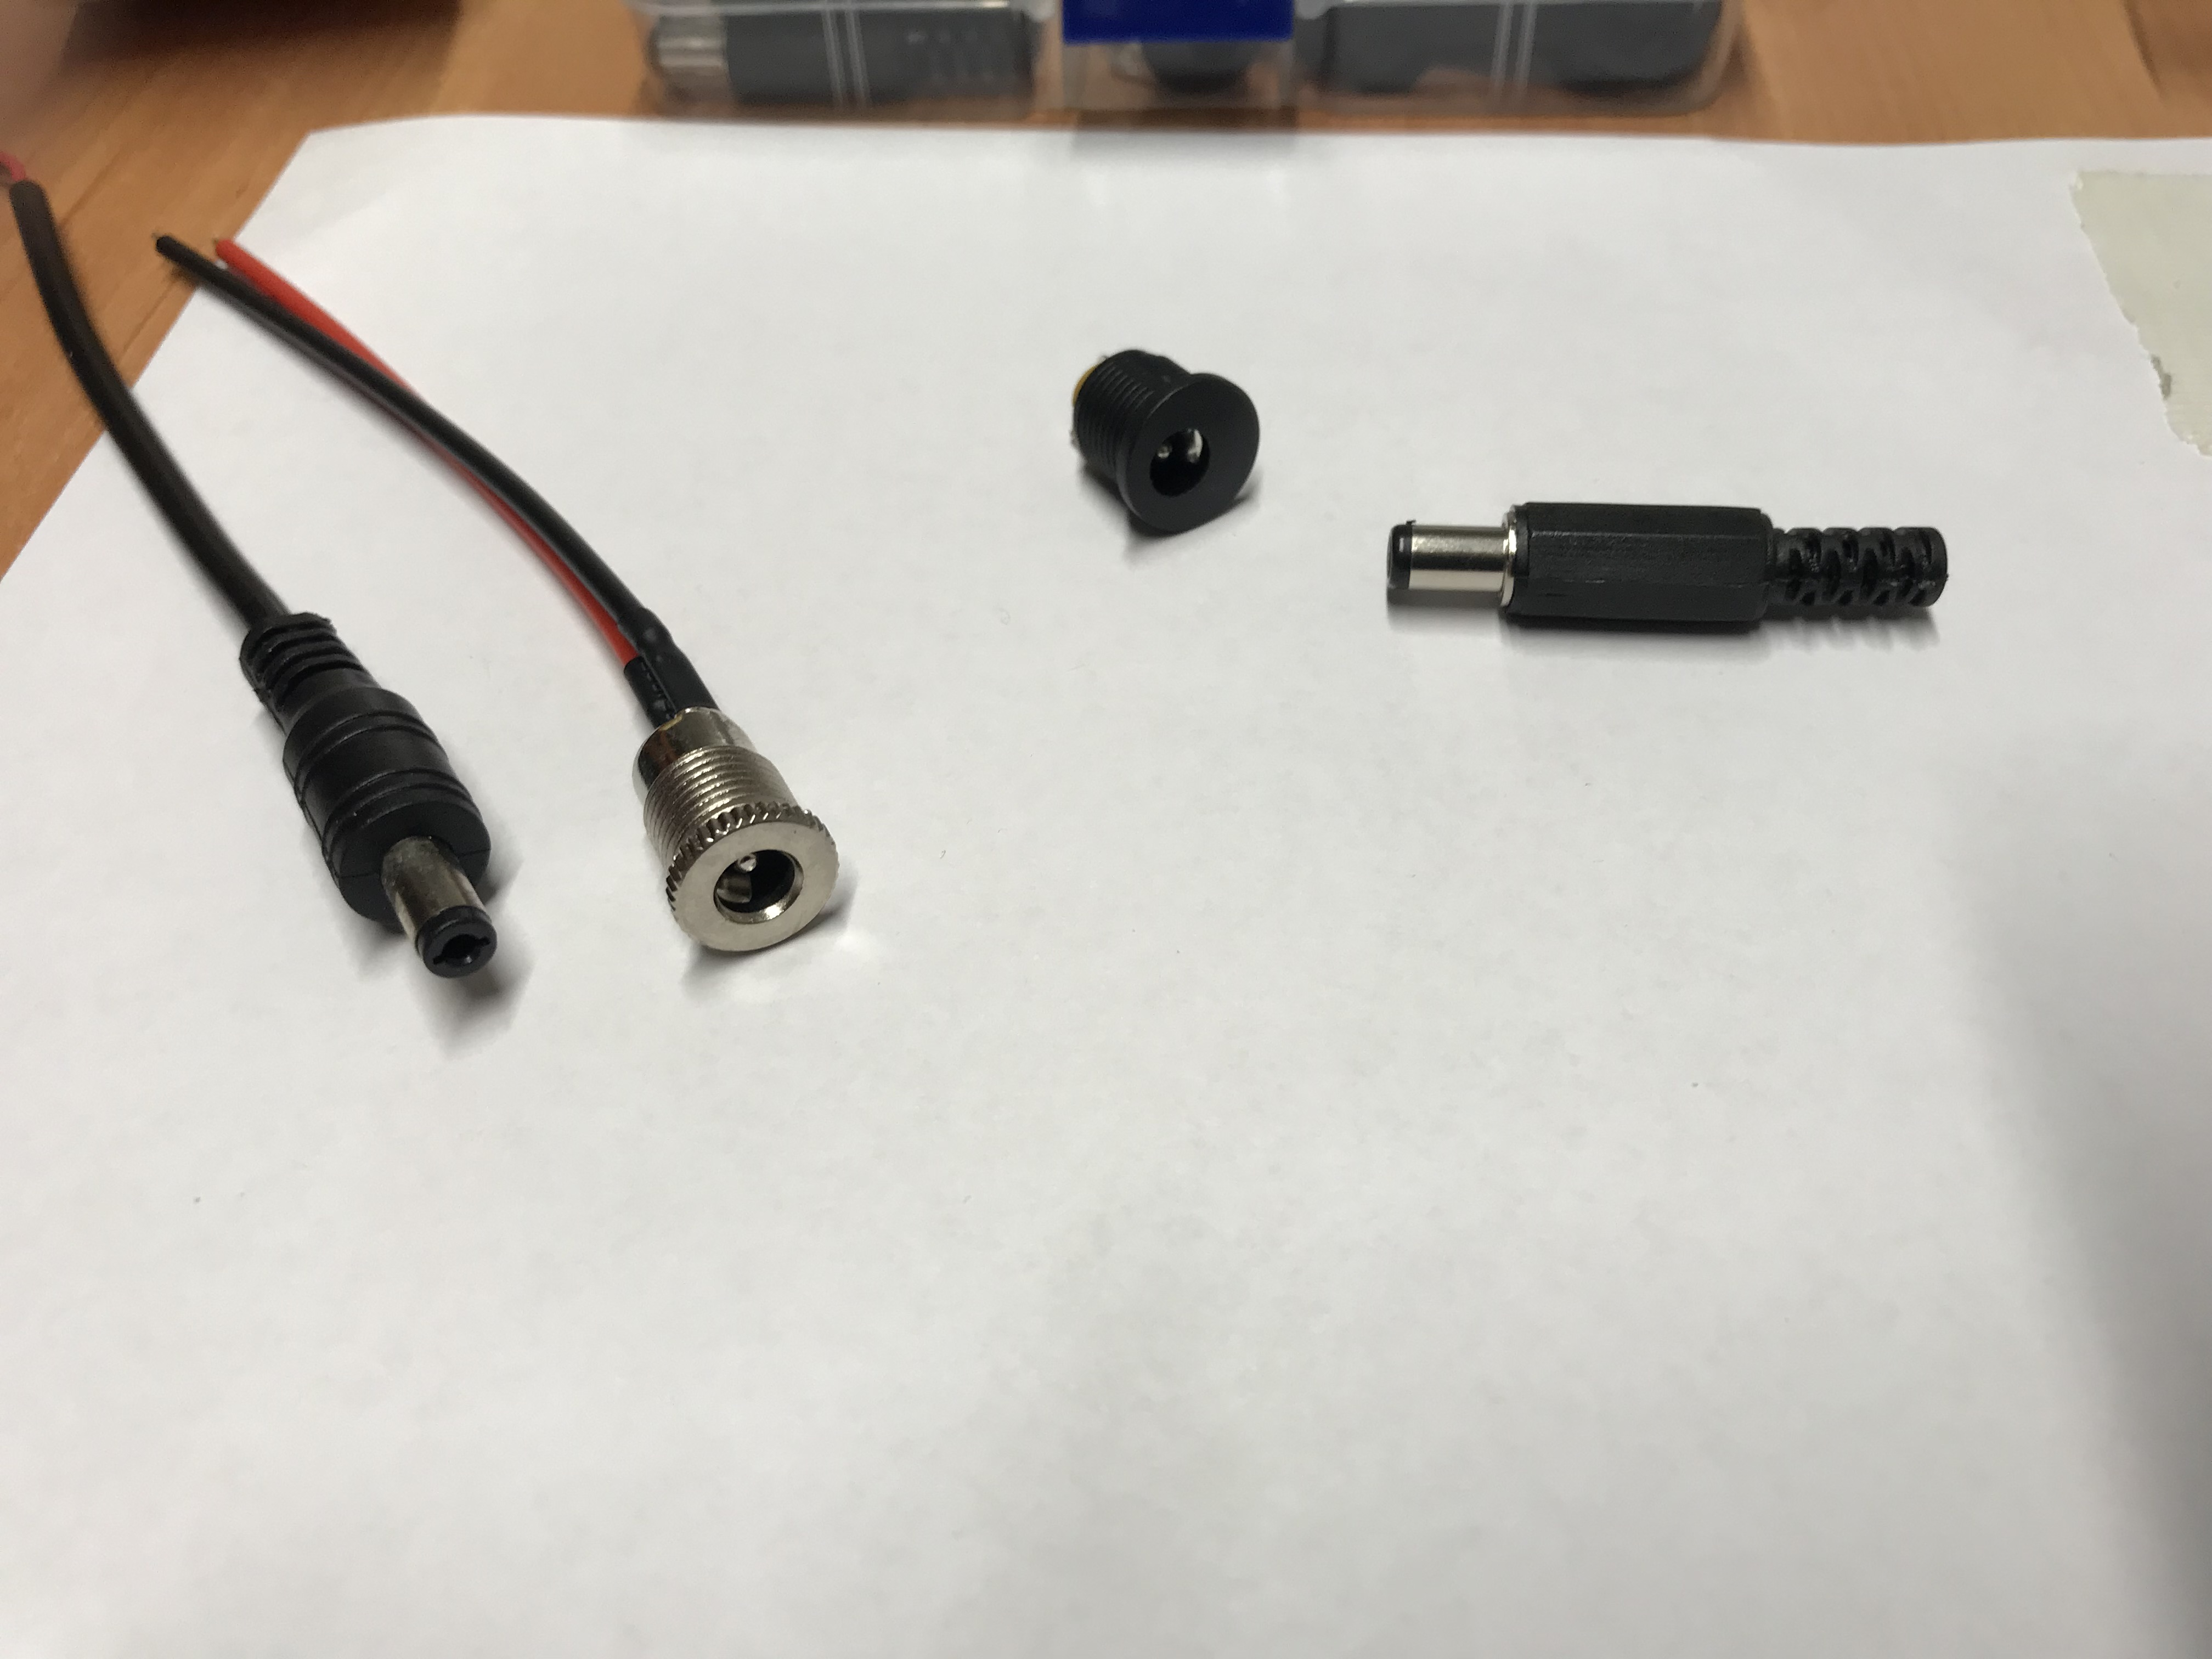
\includegraphics[scale=.05]{pictures/dcJack.jpg}};
            \end{scope}
        }{
            \draw (0,0) rectangle (3,1.5) ;
        }{Amazon}{Sin Id} {24V} {3A}

        \multicolumn{5}{|l|}{\makecell[l]{
            \tabitem Incluye tuerca para sujetar a panel \\
            \tabitem Es de metal conectado a (-) \\
            \tabitem Cables pre-soldados
        }} \\
        \hline
    \end{tabular}
    \caption{Jack 2mm Amazon}
    \label{tab:DcJack2}
\end{table}


\begin{table}[H]
    \centering
    \renewcommand\theadfont{\bfseries}
    \setlength{\tabcolsep}{10pt}
    \renewcommand{\arraystretch}{1.5}


    \begin{tabular}{c |c |c |c |c |}
        entrada & \thead[b]{item} & \thead[b]{Recomendado} & \thead[b]{Maximo} & \thead[b]{Con Bypass} \\ 
        \Xhline{5\arrayrulewidth}
%Entrada DCC
        \rowcolor{Melon!15}
        & Voltaje &14-20V & \multicolumn{2}{c|}{12-24V} \\
        \cline{2 - 5}
        \rowcolor{Melon!10} \cellcolor{Melon!15}
        \multirow{-2}{*}{DCC}&Corriente & 1A & 1.5A & 2A \\ \Xhline{3\arrayrulewidth}
%Entrada Jack
        \rowcolor{blue!15} & Voltaje & 12-20V & \multicolumn{2}{c|}{10-24V} \\
        \cline{2 - 5}
        \rowcolor{blue!10} \cellcolor{blue!15} \multirow{-2}{*}{ \makecell{ \cellcolor{blue!15} Jack\\ \cellcolor{blue!15} Terminal}} & Corriente & 1A & 1.5A & 3A \\
        \Xhline{5\arrayrulewidth}
    \end{tabular}
    \caption{Limites de entrada}
    \label{tab:limiteEntrada}
\end{table}